\documentclass{beamer}
\usetheme{default}
\usepackage{listings}
\usepackage{color}
\usepackage{hyperref}

\definecolor{dkgreen}{rgb}{0,0.6,0}
\definecolor{gray}{rgb}{0.5,0.5,0.5}
\definecolor{mauve}{rgb}{0.58,0,0.82}

\def \lstrset {\lstset{ language=R, basicstyle=\scriptsize,frame=single,
    keywordstyle=\color{blue},stringstyle=\color{mauve},commentstyle=\color{dkgreen}}}

\title{Time series in R}
\author{Andrzej Pragacz}

\begin{document}


\titlepage

\section{Theory}

\begin{frame}{White noise}
Identically indepently distributed random variables ($\epsilon_t \sim N(0, \sigma^2)$)

Can be obtained in this way:
\lstrset
\lstinputlisting{R/xts/white_noise.R}

\end{frame}


\begin{frame}{Basic time series models}
Moving-average model
$$
X_t = \mu + \epsilon_t + \Theta_1 \epsilon_{t-1} + \ldots + \Theta_q \epsilon_{t-q}
$$

Autoregressive model
$$
X_t = c + \epsilon_t + \phi_1 X_{t-1} + \ldots + \phi_p X_{t-p}
$$
Autoregressive moving-average model
$$
X_t = c + \epsilon_t + \phi_1 X_{t-1} + \ldots + \phi_p X_{t-p} + \Theta_1 \epsilon_{t-1} + \ldots + \Theta_q \epsilon_{t-q}
$$

\end{frame}


\section{xts package}

\begin{frame}{Loading and plotting time series}
loading:
\lstrset
\lstinputlisting{R/xts/loading.R}

displaying summary, plotting:
\lstrset
\lstinputlisting{R/xts/playing_around.R}
\end{frame}

\begin{frame}{SP500 Plot}
\begin{center}
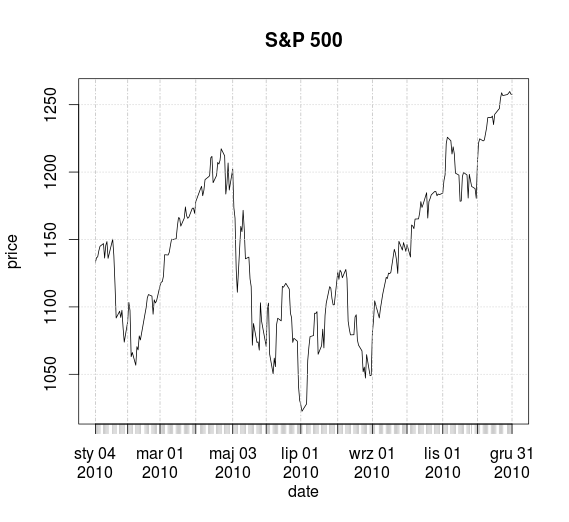
\includegraphics[width=0.8\textwidth]{img/SP500.png}
\end{center}
\end{frame}

\begin{frame}{Processing time series}

Calculating returns:
\lstrset
\lstinputlisting{R/xts/processing_returns.R}

Rolling mean / standard deviation:
\lstrset
\lstinputlisting{R/xts/processing_roll.R}
\end{frame}

\begin{frame}{Returns histogram}
\begin{center}
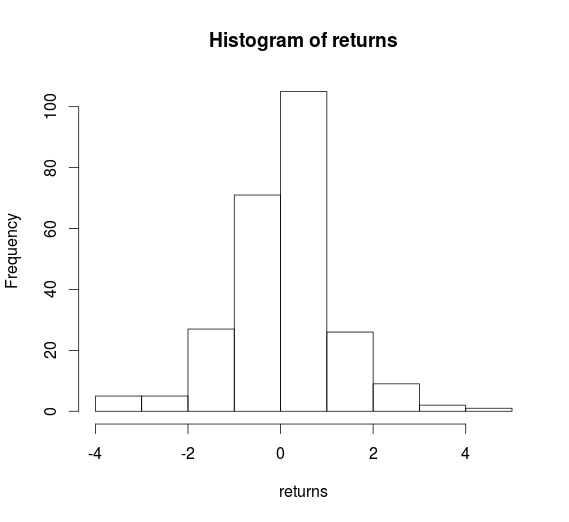
\includegraphics[width=0.8\textwidth]{img/returns_hist.png}
\end{center}
\end{frame}

\begin{frame}{Rolling mean}
\begin{center}
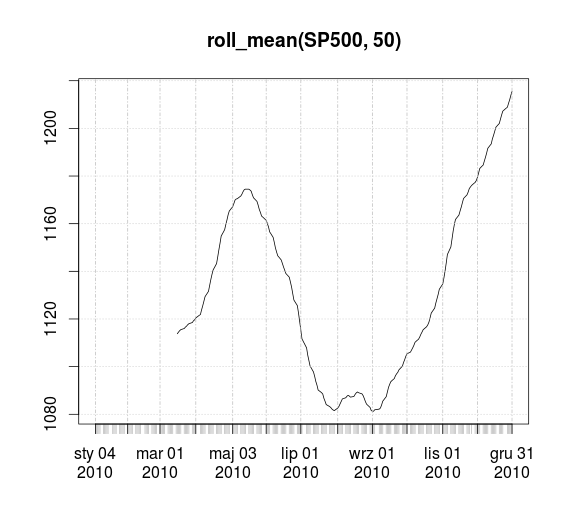
\includegraphics[width=0.8\textwidth]{img/roll_mean.png}
\end{center}
\end{frame}

\begin{frame}{Rolling standard deviation}
\begin{center}
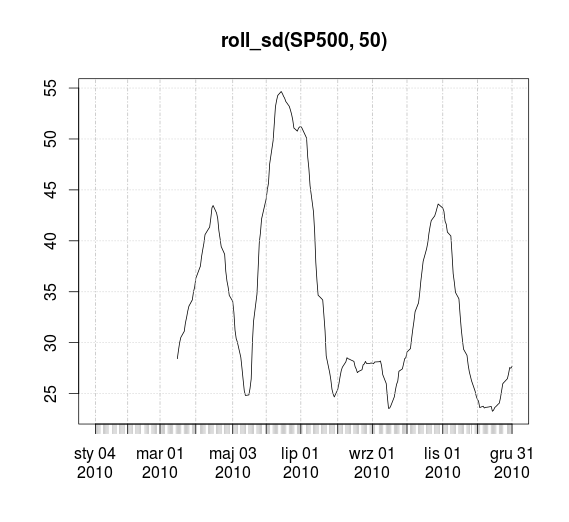
\includegraphics[width=0.8\textwidth]{img/roll_sd.png}
\end{center}
\end{frame}

\begin{frame}{Other topics}
\begin{itemize}
\item Vector Autoregression
\item Cointegration
\item Granger causality
\end{itemize}
\end{frame}

\end{document}
